\chapter[Michaelis-Menten model]{An application to systems biology: Michaelis-Menten model}

This is a model for enzyme kinetics: relates the rate of formation of a biochemical product $P$ to the concentrations of a substrate $S$ and enzyme $E$, via an intermediate complex $C$. 
\begin{gather*}
	\schemestart
	$S$ + $E$ \arrow{<=>[$k_1$][$k_2$]} $C$
	\arrow{->[$k_3$]} $E$ + $P$  
	\schemestop
\end{gather*}
Here $k_i$ are the different reaction rates. The dynamical equations for this system are:
\begin{align*}
	\frac{\md S}{\md t} &= -k_1 SE + k_2 C\\
	\frac{\md E}{\md t} &= -k_1 SE + k_2 C + k_3 C \\
	\frac{\md C}{\md t} &= k_1 SE - k_2 C - k_3 C \\
	\frac{\md P}{\md t} &= k_3 C
\end{align*}
The system is quadratic nonlinear due to the presence of $SE$. Note that
\begin{gather*}
	\frac{\md}{\md t} (E+C) = 0 \qquad \implies E + C = E_0
\end{gather*}
since the total amount of initial enzyme remains the same. Further, there is no complex or product initially. Our initial conditions are therefore
\begin{align*}
	E(0) &= E_0 \\
	S(0) &= S_0 \\
	C(0) &= 0 \\
	P(0) &= 0
\end{align*}  
Since $E(t) = E_0 - C(t)$, we are left with three coupled equations. Now the natural small parameter in this system is 
\begin{gather*}
	\epsilon = \frac{E_0}{S_0} \ll 1
\end{gather*}
as is often the case (though not always). This allows us to simplify the problem significantly. We are typically interested in the effective rate law for the production of $P$, i.e. a simple formula for $\md P/\md t$ in terms of the known rate constants $k_i$ and $S_0$. Let us first non-dimensionalize the sytem using
\begin{align*}
	s &= \frac{S}{S_0} \qquad p = \frac{P}{S_0} \\
	e &= \frac{E}{E_0} \qquad c = \frac{C}{E_0} 
\end{align*}
with $0 \leq s,p,e,c\leq 1$. {\color{red} [Check]} Why can't $p>1$? Our coupled system now reads:
\begin{align*}
	\frac{\md s}{\md t} &= -{k_1 E_0} s(1-c) + k_2 \frac{E_0}{S_0} c \\
	\frac{\md c}{\md t} &= k_1 S_0 s (1-c) - (k_2+k_3) c 
\end{align*}
using $e+c=1$. Note that we do not need the evolution equation for $P$ to solve the coupled sub-system $S$ and $C$. Now $k_1 E_0$ must have the units of $1/t$. So we introduce the dimensionless time 
\begin{gather*}
	\tau = k_1 E_0 t
\end{gather*}
which leads to the governing equation set
\begin{align*}
	\frac{\md s}{\md \tau} &= -s(1-c) + \underbrace{\frac{k_2}{k_1 S_0}}_\lambda c \\
	\frac{\md c}{\md \tau} &= \frac{1}{\epsilon} s (1-c) - \frac{1}{\epsilon} \underbrace{\frac{k_2+k_3}{k_1 S_0}}_\mu  c \\
	& s(0) = 1 \qquad c(0)=0
\end{align*}
For posterity also note
\begin{gather*}
	\frac{\md p}{\md \tau} = \underbrace{\frac{k_3}{k_1 S_0}}_{\mu -\lambda} c
\end{gather*}
Now there are two ways to analyze this problem. 
\paragraph{Phase-plane analysis} Recall our equations
\begin{align*}
	s' &= -\left[s(1-c) - \lambda c\right] \\
	c' &= \frac{1}{\epsilon} \left[s(1-c) - \mu c\right]
\end{align*}
Since the concentration of the intermediate complex is not expected to change in the steady-state, we examine the $c'=0$ state in the first quadrant (concentrations are positive). This yields the quasi--steady state approximation
\begin{gather*}
	s = \frac{\mu c}{1-c}
\end{gather*} 
In perturbation theory terms this is the \underline{outer} solution. The initial concentration is $(s,c)=(1,0)$. Here
\begin{align*}
s' = -1 \qquad c' = \frac{1}{\epsilon} 
\end{align*}
which means the horizontal component varies rapidly except in an $O(\epsilon)$ neighborhood of $c'=0$ where $c'=O(1)$ and comparable to $s'$. On the curve $c'=0$, we can only move downwards. It can be further shown that anywhere other than the $O(\epsilon)$ region of $c'=0$, the vector field would push the phase-space points back onto the curve {\color{red} [To do]}. 
\begin{figure}[!h]
	\centering
	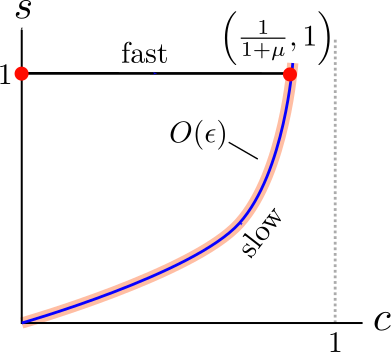
\includegraphics[width=0.5\textwidth]{./plots/pdf/MichaelisMenten.pdf}
	\caption{The $O(\epsilon)$ neighborhood is shown in orange about the quasi steady-state solution $c'=0$ shown in blue.}
	\label{fig:strogatz-wk17}
\end{figure}

\paragraph{Perturbative approach} Let us look at the \emph{fast} variation. Define an inner ``rapid'' time scale
\begin{gather*}
T = \frac{\tau}{\epsilon}
\end{gather*} 
This yields
\begin{align*}
\frac{\md s}{\md T} &= -\epsilon s(1-c) + \lambda \epsilon c \\
\frac{\md c}{\md T} &= s(1-c) - \mu c
\end{align*}
Proceeding with our usual anstaz, the lowest order equations are:
\begin{align*}
\frac{\md s_0}{\md T} &= 0 \\
\frac{\md c_0}{\md T} &= s_0 (1-c_0) - \mu c_0
\end{align*}
With our initial conditions
\begin{align*}
s(0) = 1 &= s_0 + \epsilon s_1 + \dots \\
c(0) = 0 &= c_0 + \epsilon c_1 + \dots 
\end{align*}
we find
\begin{align*}
s_0(T) & = 1 \\
c_0(T) &= \frac{1 - \me^{-(\mu+1)T}}{1+\mu} \\
\implies c(T\rightarrow \infty) &= \frac{1}{1+\mu}
\end{align*}
Now the intermediate complex in steady state does not change its concentration, i.e. $\md c/\md T = 0$. This also yields
\begin{align*}
c(T) &\approx \frac{s(T)}{\mu + S(T)} \\
c_0(T) &\sim  \frac{s_0}{\mu + s_0} =  \frac{1}{\mu + 1}
\end{align*}
Finally, the rate of product formation (except for the initial transient) is
\begin{align*}
\frac{\md p_0}{\md \tau } = (\mu -\lambda) \frac{s_0}{\mu + s_0} = - \frac{\md s_0}{\md \tau }
\end{align*}
The above is referred to as the ``Michaelis-Menten kinetics''. 
